\subsection{Rancangan Detail In-Memory Store}
\label{subsection:detail-in-memory-store}

Komponen \textit{In-Memory Store} bertanggung jawab untuk menyimpan data secara sementara dalam memori. Komponen ini akan menggunakan struktur data yang sesuai untuk memastikan bahwa data dapat disimpan dan diambil dengan cepat. Sesuai dengan bagian \ref{subsubsection:in-memory-kv-store}, komponen ini menggunakan Moka sebagai sistem \textit{cache}. Rancangan komponen dapat dilihat pada gambar \ref{fig:in-memory-store-component}.

\begin{figure}[ht]
    \centering
    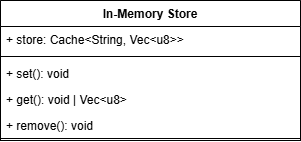
\includegraphics[width=0.4\textwidth]{resources/chapter-3/in-memory-store-component.png}
    \caption{Struktur Komponen In-Memory Store}
    \label{fig:in-memory-store-component}
\end{figure}